



Once we debug the interfaces between the methods of \tbl{overview}, then we will be able to
code up multile ``SLR workflows'' that use different subsets of \tbl{overview}.
\fig{workflow} shows examples of three such workflows. 
The core question of this work is this:  is the added complexity of more complex workflows
necessary? To answer this question, researchers using our infrastructure will perform and repeat literature reviews. From  that  data  we  will  be  able  to  comment  on  value-added  (if  it  exists)  of  the more
complex workflow versus  doing something fully manual (like Workflow(a) in \fig{workflow}) or something somewhat more intricate (like Workflow(b) in \fig{workflow}).


{\IT} will be seen to be a  success
when the toolkit can conclude that   SLR workflow1 is ``better than'' workFlow2 (where ``better'' is defined below).
Note that such a conclusion would need to be based on results of dozens of literature reviews.  
To find those reviews, we will lever
the community nature of this work.
Since we plan to acquire a large number of SLRs
from our collaborators, we will have access to numerous SLR case studies-- some of which 
repeat prior SLRs. This will   allow us to compare the results of {\IT}'s manual+automatic methods
against traditional methods. 
Other SLRs will be for new research questions, thus allowing us
to understand the ease (or otherwise) of applying {\IT} to new domains.

\begin{figure}[!b]
    \centering
    \subfloat[An example workflow for searching and selection, following the current practice of manual SLRs~\cite{jalali2012systematic}.]
    {
        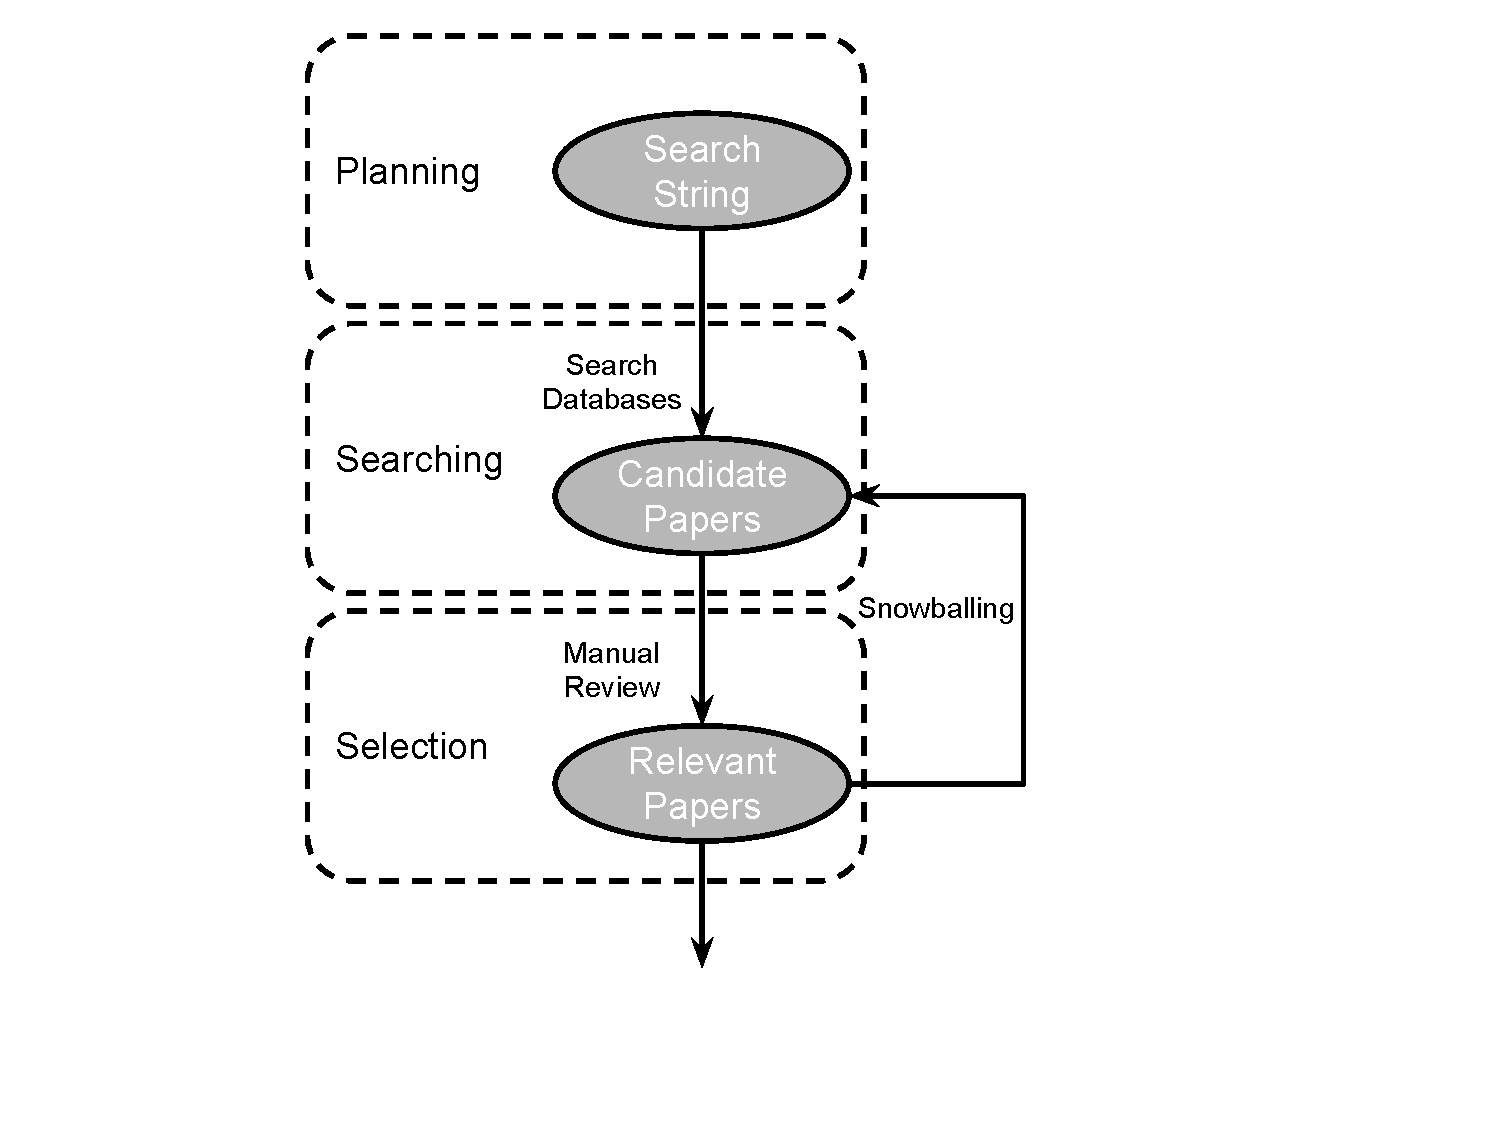
\includegraphics[width=0.30\linewidth]{workflow1.pdf}
    }\quad
    \subfloat[An example workflow for searching and selection, applying text mining and active learning tools to SLRs~\cite{Yu2018,Yu2019}.]
    {
        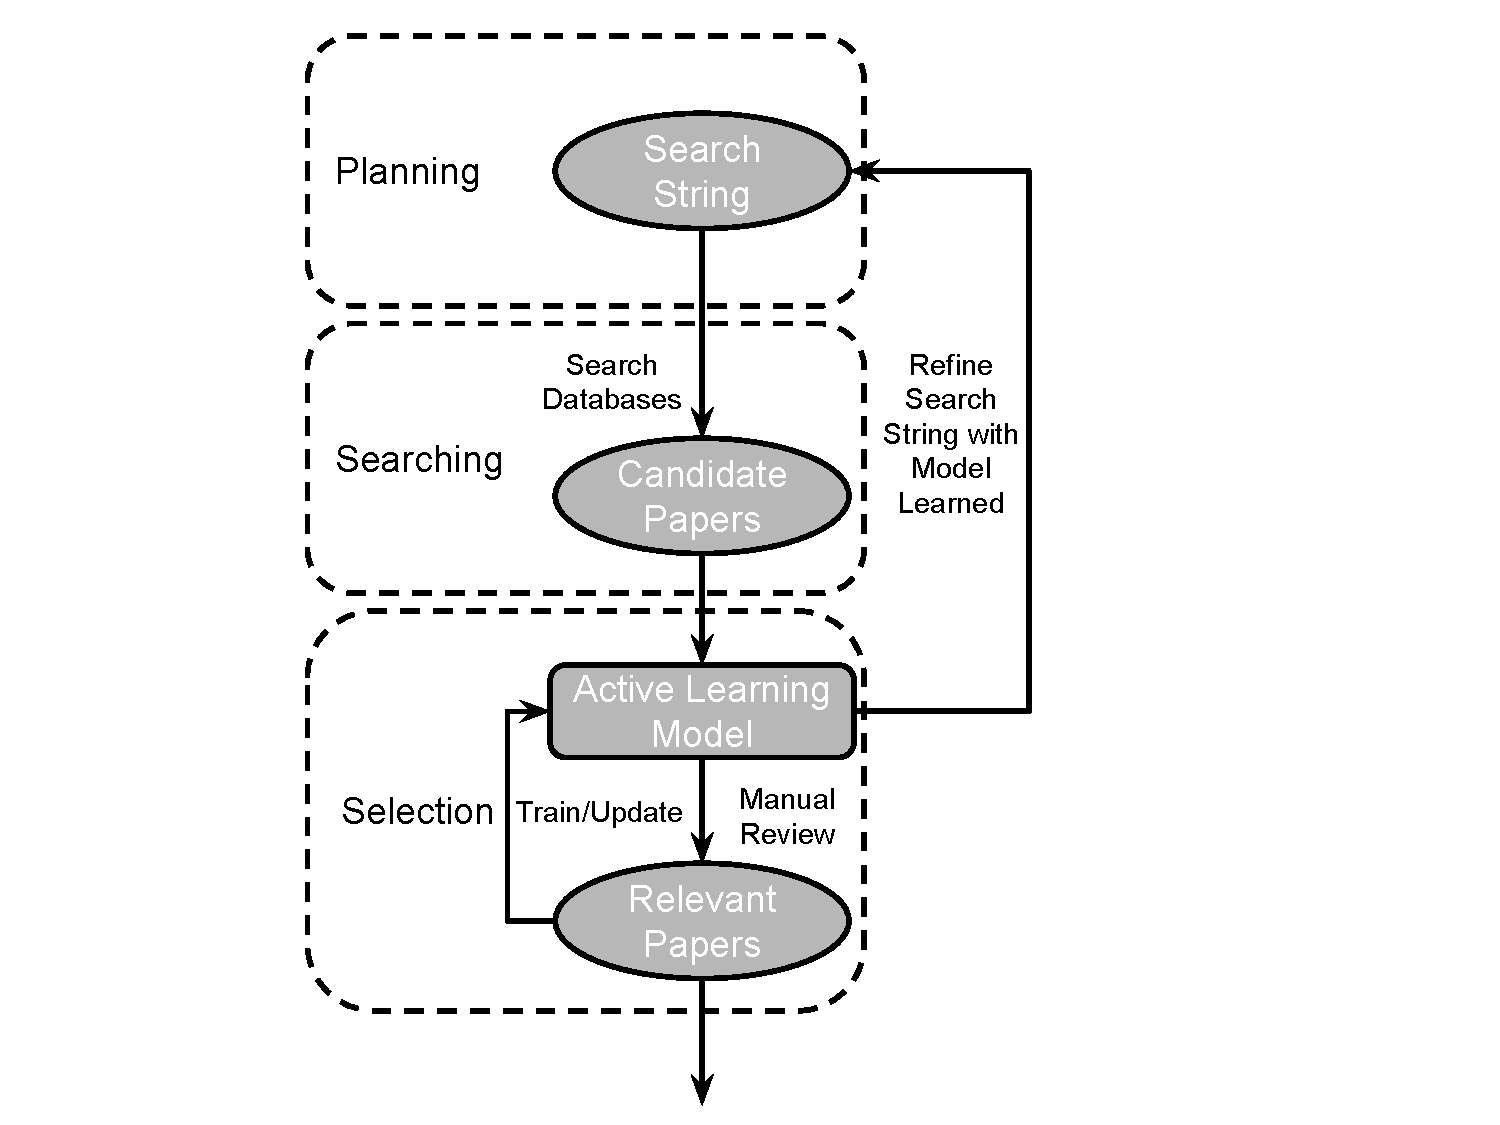
\includegraphics[width=0.31\linewidth]{workflow2.pdf}
    }\quad
    \subfloat[An example workflow for searching and selection, which combines Workflow(a) and (b).]
    {
        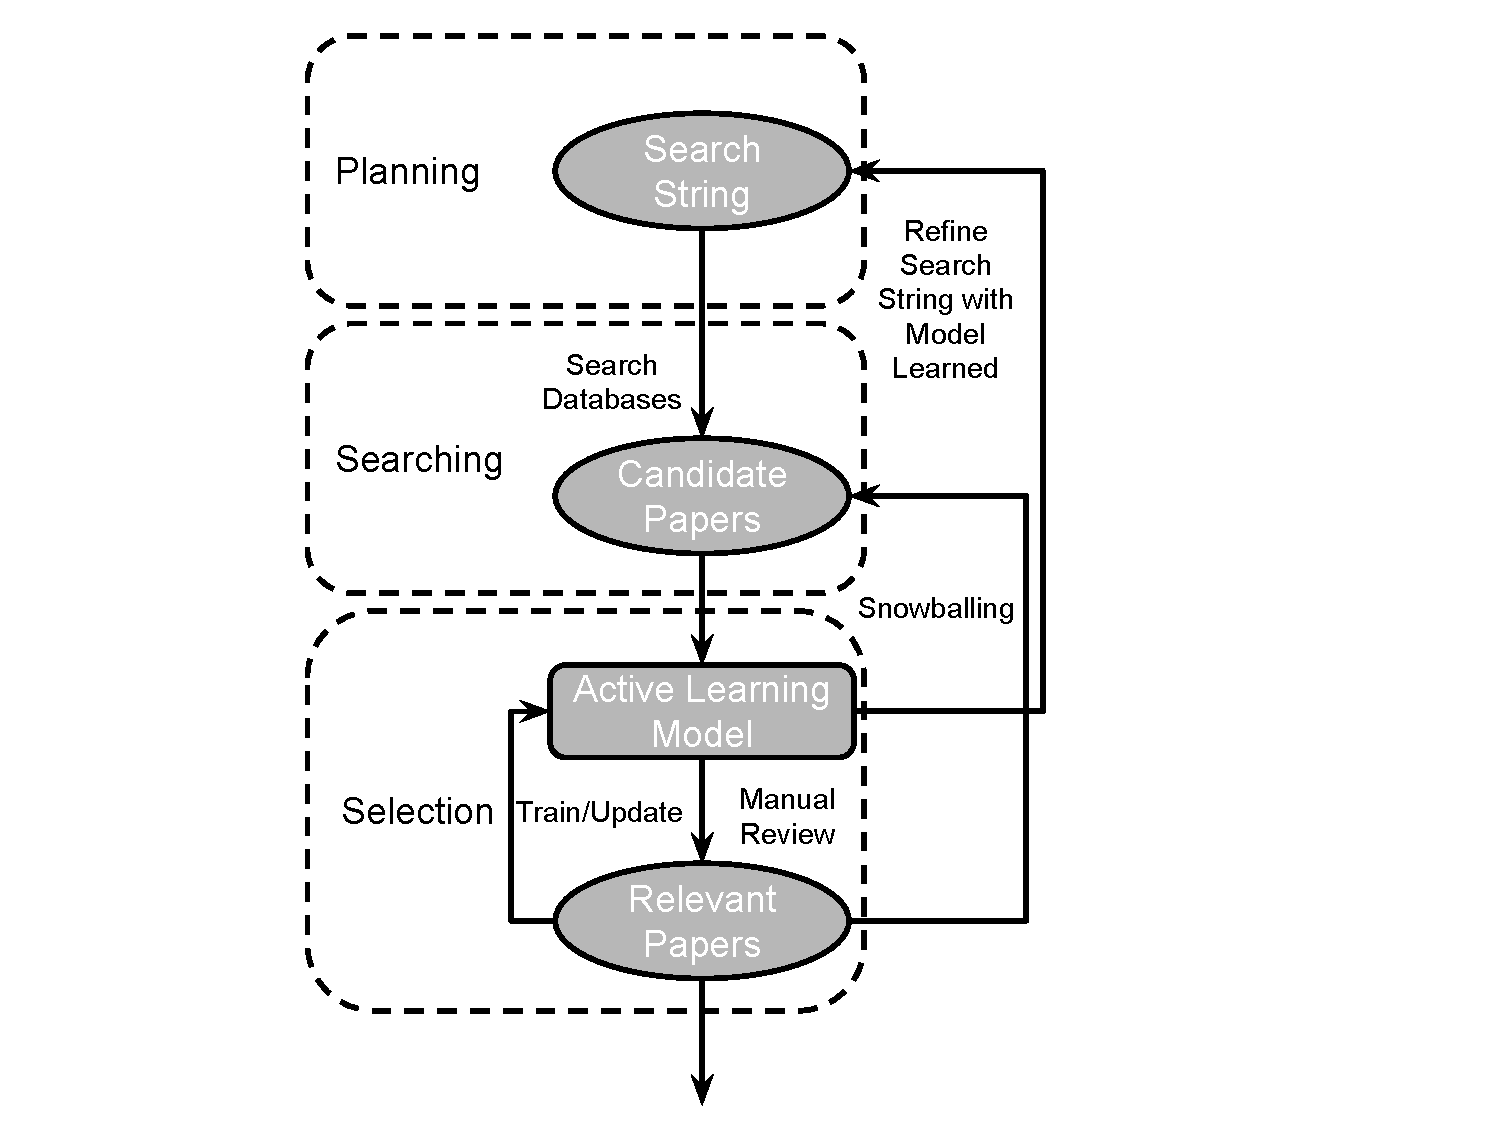
\includegraphics[width=0.295\linewidth]{workflow3.pdf}
    }
    \caption{Example alternative workflows for searching and selection where Workflow(c) = Workflow(a) + Workflow(b).}
    \label{fig:workflow}
\end{figure}

\noindent
We will say that 
Workflow1 is ``better'' than Worfkflow2 if the methods in Workflow1 are:
\begin{enumerate}[itemsep=0pt,parsep=0pt]
\item Easier to learn.
\item Finds more relevant
items than Workflow2 (where ``relevant'' is judged by a human being). 
\item Faster to apply. This is an important criteria since manual SLR require  days to weeks to complete.
\end{enumerate}
Other ``better'' measures include:
\begin{enumerate}[resume,itemsep=0pt,parsep=0pt]
\item
The ``return factor''; i.e. other researchers  elect to use Workflow1 not just once, but multiple times. 
\item
The ``ignore factor''; i.e. some method is in {\IT} but it is never used by researchers other than ourselves
(and ``better'' methods are ignored ``less'').
\item
The ``publication factor''; i.e. published papers based their conclusions on methods taken     {\IT}.
\end{enumerate}
Note that items 1,2,3 could be assessed in controlled laboratory settings while 4,5,6 would take months to years to collect.
Hence, for items 1,2,3, we request funds for travel to senior conference venues where we will conduct controlled experiments where current
SE researchers use our tools. Also, for items 4,5,6 we request funds for a multi-year project.
\vspace{8pt}

We intend to perform both formative and summative evaluation of the proposed infrastructure. 
This section describes each of those evaluations in detail.
\vspace{8pt}

\subsection{Formative Evaluation}
Formative evaluation will help ensure that we are developing the most appropriate infrastructure for the various stakeholders described in Figure~\ref{figure-ResearchEnabled}.
During development of the infrastructure, we will interact with key stakeholders (through workshops and one-on-one sessions at various conference venues) to ensure that the infrastructure will meet their needs.

First, we will have ongoing interactions with members of the Software Engineering research community, including Empirical Software Engineering Researchers and Text Mining Researchers.
These researchers are key to the formative evaluation because we must ensure that the design of our infrastructure can enable the types of research these communities would like to conduct.
We will seek input from members of these communities both early in the process, to inform our design, as well as throughout development to ensure the infrastructure is meeting their needs.

Second, early in the project, we will conduct a community workshop. 
The goal of this workshop will be to ensure that we are on course to realize value from the implementation of the {\IT} infrastructure. 
During the workshop we will demo the various tools we have developed to that point give workshop attendees an opportunity to interact directly with those tools. 
The workshop will provide opportunities for community members to discuss their perspectives and provide feedback once they have reviewed the status of the {\IT} functionality.  
Our desire is to ensure the implementation is providing functionality to meet their needs.
We will specifically ask the workshop attendees to provide feedback to guide the remainder of the development effort.
\vspace{8pt}

\subsection{Summative Evaluation}
Throughout development, the summative evaluation will quantify the adoption and perceived usefulness of {\IT}.
We will gather data in four ways:
(1)~we will periodically send short surveys to infrastructure users to measure their acceptance and perceived usefulness of the infrastructure;
(2)~we will gather insights from attendees of our second community workshop, to be held at the end of the grant period, to help ensure that SLR tool developers and authors find value in {\IT}, which will be the key success trigger to ensuring its sustainability beyond the grant period; and
(3)~we will provide a citable URL so we can track how many SLRs are completed with the aid of the infrastructure. 

The second community workshop will be similar to the first community workshop.
We will invite active members of our target communities (Figure~\ref{figure-ResearchEnabled}) to participate in this interactive workshop.
We will use this time to train attendees on the current functionality of {\IT} and how to use it to perform various important SLR tasks.
We will the allow workshop attendees to use {\IT} and gather evaluation data through usage statistics and surveys to evaluate effectiveness.

